	\section{Nombre: Piso congelado}\label{obs.pisoC}
	\subsection{Descripción}
	Porción de suelo. Cuando el jugador camina sobre este obstáculo, la fricción entre el jugador y el obstáculo disminuye provocando que la velocidad de desplazamiento del jugador se incremente y que cuando el jugador se detenga no lo haga de golpe sino resbale una distancia determinada antes de detenerse.
	\subsection{Esquema}
Ver figura \ref{fig:pisoC}.
	\begin{figure}
  \centering
  \subfigure[El jugador incrementa su velocidad de desplazamiento horizontal al caminar sobre el piso congelado.]{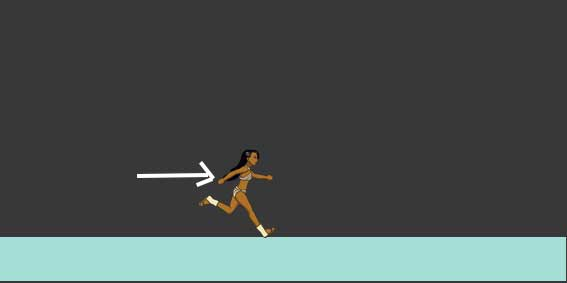
\includegraphics[width=0.3 \textwidth]{Imagenes/sueloRes}}
   \subfigure[Aunque el jugador se detiene, continua su desplazamiento por la poca fricción entre el y el suelo congelado.]{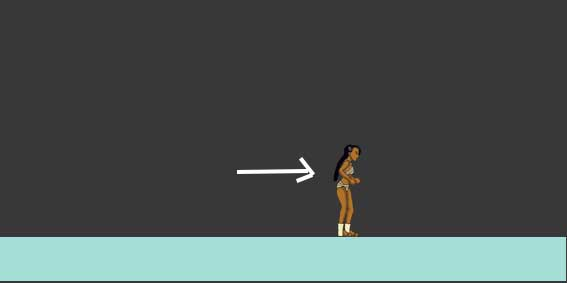
\includegraphics[width=0.3 \textwidth]{Imagenes/sueloRes02}}
  \caption{Piso congelado.}
  \label{fig:pisoC}
\end{figure} 